\section{高斯——旺策尔定理的证明梗概}
\phantomsection
\label[appendix]{app:gauss-wantzel-theorem}

%% https://math.stackexchange.com/questions/4102110/proof-of-gauss-wantzel-theorem
%% https://www.raahilmullick.com/wp-content/uploads/2024/10/SUMaC_Research_Project.pdf
%% https://mp.weixin.qq.com/s/vyDQ7wMUTOuvsomFLWcgqg

高斯——旺策尔定理的证明梗概需要复数的知识,建议读者先阅读第6章。这一定理给出了正$n$边形可用尺规作出的\underdot{充分必要}条件。即$n=2^k p_1 p_2 \dotsm p_m$其中$p_i$是彼此不同的费马素数。

\subsection{域}
我们首先引入域的概念。这是抽象代数中的一个重要概念,可以帮助我们把所有尺规可作出数的范围严格地界定出来。在历史上,第一个明确使用这个概念的人是法国数学天才伽罗瓦,但是他没有给这个概念命名。1871年,德国数学家戴德金给出了域的德语名字körper\footnote{中文译作“体”,例如范·德·瓦尔登《代数学》的中译本。},其对应的英文为field。

\begin{definition}
一个集合$\mathbf{F}$叫做域,如果它上面定义了加法和乘法两种运算,并且满足如下条件:
\begin{enumerate}[(1)]
\item 结合律。加法、乘法都满足结合律,即:
  \begin{align*}
    a + b + c &= a + (b + c) \\
    abc &= a(bc)
  \end{align*}

\item 交换律。加法、乘法都满足交换律,即:
  \begin{align*}
    a + b &= b + a \\
    ab &= ba
  \end{align*}

\item 分配律,即:$(a + b)c = ac + bc$。由于满足交换律,所以$c(a + b) = ca + cb$也成立。
\item 加法有单位元0,乘法有单位元1(见第\ref{sec:unit}节),并且$0 \ne 1$,即:
\[
a + 0 = 0 + a = a \qquad a1 = 1a = a
\]

\item 加法存在逆,即对$\mathbf{F}$中任何元素$a$,存在$b$使得:
\[
a + b = b + a = 0
\]
这个条件本质上定义了减法。

\item 对任何非零元素,乘法存在逆,即对任何$\mathbf{F}$中的元素$a \ne 0$,存在$b$使得:
\[
ab = ba = 1
\]
这个条件本质上定义了除法。
\end{enumerate}
\end{definition}

读者也许看出来了:域就是可以做加减乘除四则运算的集合。例如, 全体有理数$\mathbb{Q}$是一个域;全体实数$\mathbb{R}$是一个域;全体复数$\mathbb{C}$是一个域。我们还能找到更精细的域么?例如比有理数域大,但比实数域小?为此我们引入记号$\mathbb{Q}(\sqrt{a})$,其中$a$为不含平方因子的正整数。我们用例子$\mathbb{Q}(\sqrt{2})$来解释一下这个符号。它是所有形如

\be
x = a_0 + a_1 x + a_2 x^2 + \dotsb + a_n x^n
\ee
的多项式,当$x = \sqrt{2}$时得出的数构成的集合。其中$a_0, a_1, a_2, \dotsc, a_n$都是有理数。代入$\sqrt{2}$就是:

\be
x = a_0 + a_1 \sqrt{2} + a_2 (\sqrt{2})^2 + \dotsb + a_n (\sqrt{2})^n
\label{eq:polynomial-sqrt2}
\ee

这个数看似吓人,其实是个“纸老虎”。因为$(\sqrt{2})^2 = 2$是有理数,$(\sqrt{2})^4, (\sqrt{2})^6, \dotsc$都是有理数;$(\sqrt{2})^3 = 2\sqrt{2}$是$a\sqrt{2}$的形式,$(\sqrt{2})^5 = 4\sqrt{2}$是$a\sqrt{2}$的形式……所以\ref{eq:polynomial-sqrt2}的所有奇数项都是有理数$p_i$,所有的偶数项都是$q_i\sqrt{2}$,合并同类项后得:

\[
x = p + q\sqrt{2}
\]

其中$p, q$都是有理数,也就是说$\mathbb{Q}(\sqrt{2})$含有所有形如$p + q\sqrt{2}$的数,并且:

\begin{proposition}
所有形如$p + q\sqrt{2}$的数经过加减乘除四则运算后仍然在$\mathbb{Q}(\sqrt{2})$内,其中$p, q$是有理数。
\end{proposition}

\begin{proof}
加减法的结果为$a + b\sqrt{2} \pm (c + d\sqrt{2}) = (a \pm c) + (b \pm d)\sqrt{2}$,仍然是$p + q\sqrt{2}$的形式,在$\mathbb{Q}(\sqrt{2})$内。

乘法的结果为$(a + b\sqrt{2})(c + d\sqrt{2}) = (ac + 2bd) + (bc + ad)\sqrt{2}$,仍然是$p + q\sqrt{2}$的形式,在$\mathbb{Q}(\sqrt{2})$内。

除法的结果为

\begin{align*}
\frac{a + b\sqrt{2}}{c + d\sqrt{2}} &= \frac{(a + b\sqrt{2})(c - d\sqrt{2})}{(c + d\sqrt{2})(c - d\sqrt{2})} &&\text{分子分母同乘}c - d\sqrt{2} \\
&= \frac{(ac - 2bd) + (bc - ad)\sqrt{2}}{c^2 - 2d^2} &&\text{平方差公式} \\
&= \frac{ac - 2bd}{c^2 - 2d^2} + \frac{bc - ad}{c^2 - 2d^2}\sqrt{2}
\end{align*}
仍然是$p + q\sqrt{2}$的形式,在$\mathbb{Q}(\sqrt{2})$内。
\end{proof}

这就证明了$\mathbb{Q}(\sqrt{2})$是一个域。这个域有什么特殊之处呢?我们知道方程$x^2 - 2 = 0$在有理数域上无解,即不存在任何有理数$q$满足这个方程。但是它却在$\mathbb{Q}(\sqrt{2})$上有解$x_{1, 2} = \pm \sqrt{2}$。把无理数$\sqrt{2}$“加入”有理数$\mathbb{Q}$后,域扩大了。这说明域有大小,并且:

\[
\mathbb{Q} \subset \mathbb{Q}(\sqrt{2}) \subset \mathbb{R} \subset \mathbb{C}
\]

用尺规作出长为$\sqrt{2}$的线段(边长为1的正方形的对角线)后,再用尺规进行加减乘除运算(见第\ref{sec:geometric-arthimetic}节)能作出的所有长度就是集合$\mathbb{Q}(\sqrt{2})$。给定长度$a$,由于我们能用尺规作出$\sqrt{a}$长的线段(见命题\ref{thm:sqrt-a}),所以能获得域$\mathbb{Q}(\sqrt{a})$。

第二个重要的意义在于,把无理数$\sqrt{2}$加入有理数$\mathbb{Q}$后,“维度”变了。有理数只有一个维度:$\{q | q \in \mathbb{Q}\}$,而$\mathbb{Q}(\sqrt{2})$有两个维度:$\{p + q \sqrt{2} | p, q \in \mathbb{Q}\}$,我们需要两个变量$p, q$才能确定一个值,维度扩大了2倍。我们用符号:

\[
[\mathbb{Q}(\sqrt{2}) : \mathbb{Q}] = 2
\]

来定量表示扩大了多少。不难想象,我们用尺规作出$\sqrt{3}$,把它加入$\mathbb{Q}(\sqrt{2})$后,域$\mathbb{Q}(\sqrt{2})(\sqrt{3})$是这样的数组成的集合:

\begin{align*}
  \mathbb{Q}(\sqrt{2})(\sqrt{3}) &= \{a + b \sqrt{3} | a, b \in \mathbb{Q}(\sqrt{2}) \} \\
  &= \{p + q \sqrt{2} + (r + s\sqrt{2})\sqrt{3} \} && a, b \text{都形如} p + q\sqrt{2} \\
  &= \{p + q \sqrt{2} + r\sqrt{3} + s\sqrt{6} \}
\end{align*}

有4个变量,维度是4。我们看到维度又扩大了2倍。它相当于把两个无理数$\sqrt{2}, \sqrt{3}$加入有理数域的结果,简写成$\mathbb{Q}(\sqrt{2}, \sqrt{3})$。我们把这样的过程叫做\underdot{扩域}。注意到尺规作图的过程,就是一轮一轮扩域的过程:不断解二次方程,把$\sqrt{a}, \sqrt{b}, \dotsc$加入,构成一个扩域链:

\be
\mathbb{Q} \subset K_1 \subset K_2 \subset \dotsb \subset K_m
\label{eq:tower-of-geometric-field-ext}
\ee

但不管怎样,尺规作图每次只能把维度扩大2倍,总有$[K_{i+1} : K_i] = 2$,所以$[K_m : \mathbb{Q}] = 2^m$。读者朋友们,从维度的角度出发,$\mathbb{Q}(\sqrt[3]{2})$在这个扩域链中么?你能就此推翻倍立方问题么?(见\cref{fig:double-cube})

\begin{figure}[htbp]
 \centering
 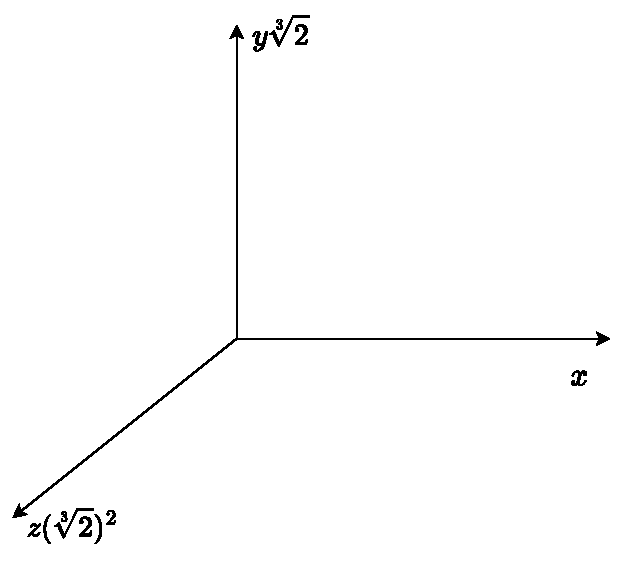
\includegraphics[scale=0.5]{../img/double-cube}
 \caption{多项式$a_0 + a_1\sqrt[3]{2} + a_2(\sqrt[3]{2})^2 + \dotsb + a_n(\sqrt[3]{2})^n$合并同类项后可表示为$p + q\sqrt[3]{2} + r(\sqrt[3]{2})^2$。故$[\mathbb{Q}(\sqrt[3]{2}) : \mathbb{Q}] = 3$,不在尺规作图的扩域链中。}
 \label{fig:double-cube}
\end{figure}

\subsection{分圆方程}
高斯将正$n$边形尺规作图的问题转化为把单位圆的圆周$n$等分问题,再利用复数进一步转化为求方程$x^n - 1 = 0$的全部复数根的问题,这种特殊的方程名叫“分圆方程”(cyclotomic equation),$n$次分圆方程有$n$个复数根:$\zeta_0 = 1, \zeta_1, \dotsc, \zeta_{n-1}$,任何$\zeta_k$满足$(\zeta_k)^n = 1$,所以又叫做$n$次单位根。根据高中学习的棣莫佛定理,可以用三角函数表示单位根:

\be
\zeta_k = e^{\frac{2k\pi}{n}} = \cos(\frac{2k\pi}{n}) + i\sin(\frac{2k\pi}{n})
\ee

从这个角度我们就能理解为何这$n$个根均匀分布在单位圆周上,并且第一根$\zeta_0 = \cos(0) + i\sin(0) = 1$。如果每个单位根都能用尺规作出(从0到$\zeta_k$代表的线段),就能作出对应的正$n$边形(例如作出$\zeta_1 - 1$,以此长度在单位圆上连续截取$n$次)。这样问题就进一步转化为判断$n$次单位根是否都在扩域链\cref{eq:tower-of-geometric-field-ext}中的问题。由于1是一个根,我们知道多项式$x^n - 1$必然有一个因子$x - 1$。下表列出了前6个多项式$x^n - 1$在有理数域上的因式分解,我们把每个首次出现在有理数域上不可进一步分解的多项式叫做$n$次分圆多项式,记作$\Phi_n(x)$。

\begin{align*}
x - 1 &= x - 1 & \Phi_1(x) &= x - 1 \\
x^2 - 1 &= (x - 1)(x + 1) & \Phi_2(x) &= x + 1 \\
x^3 - 1 &= (x - 1)(x^2 + x + 1) & \Phi_3(x) &= x^2 + x + 1 \\
x^4 - 1 &= (x^2 - 1)(x^2 + 1) = (x - 1)(x + 1)(x^2 + 1) & \Phi_4(x) &= x^2 + 1 \\
x^5 - 1 &= (x - 1)(x^4 + x^3 + x^2 + 1) & \Phi_5(x) &= x^4 + x^3 + x^2 + 1 \\
x^6 - 1 &= (x - 1)^2(x^2 + x + 1)(x^2 - x + 1) & \Phi_6(x) &= x^2 - x + 1 \\
\dotso
\end{align*}

1772年,欧拉首先发现了$x^n - 1$在有理数上的因式分解方法\cite{LinKailiang-2025}:

\be
x^n - 1 = \Phi_1(x)\Phi_a(x)\Phi_b(x) \dotsm \Phi_d(x)
\ee

其中$a, b, \dotsc, d$是所有$n$的因子,$\Phi_i(x)$是第$i$个分圆多项式。例如4的因子有1, 2, 4,所以$x^4 - 1 = \Phi_1(x)\Phi_2(x)\Phi_4(x)$;18的因子有1, 2, 3, 6, 9,18,所以$x^{18} - 1 = \Phi_1(x)\Phi_2(x)\Phi_3(x)\Phi_6(x)\Phi_9(x)\Phi_{18}(x)$。最特殊的情况发生在$n$为素数$p$时,1801年高斯证明了$p$次分圆多项式$\Phi_p(x) = x^{p-1} + \dotsb + x + 1$不可约(不能在有理数域上因式分解)。而素数$p$只有两个因子$1, p$,所以$x^p - 1 = \Phi_1(x)\Phi_p(x) = (x - 1)(x^{p-1} + \dotsb + x + 1)$。

\subsection{欧拉总计函数}
我们回到要解决的问题:判断正$n$边形能否尺规作出,只需要判断$n$次单位根是否都在扩域链\cref{eq:tower-of-geometric-field-ext}中。这意味着对任何$n$次单位根$\zeta_i$,存在某个扩域$K_m = \mathbb{Q}(\zeta_i)$。这样$\zeta_i$就可以表示成一系列二次方程的解,从而可以尺规作出。由于$[K_m : \mathbb{Q}] = 2^m$,即$[\mathbb{Q}(\zeta_i) : \mathbb(Q)] = 2^m$,所以我们只要判断把根$\zeta_i$加入有理数域$\mathbb{Q}$后,维度是否扩大了2的整数次幂就可以了。好消息是,我们无需逐一检查$\zeta_0, \zeta_1, \dotsc, \zeta_{n-1}$,例如:

\begin{enumerate}[(1)]
\item 方程$x^3 - 1 = 0$有三个根$1, \dfrac{-1 \pm i\sqrt{3}}{2}$。根$\zeta_0 = 1$是有理数。我们可以跳过根$\zeta_2 = \dfrac{-1 - i\sqrt{3}}{2}$,因为一旦把$\zeta_1 = \dfrac{-1 + i\sqrt{3}}{2}$加入有理数域$\mathbb{Q}$后,就有$\zeta_2 \in \mathbb{Q}(\zeta_1)$了(因为任何$a + b \zeta_2$都可以表示成$(a - b) - b \zeta_1$,读者可以进一步验证$\zeta_2 = \zeta_1^2$)。这三个根中,只有两个是独立的,我们把$\{1, \zeta_1\}$加入有理数域进行扩域:

\begin{align*}
[\mathbb{Q}(1, \zeta_1) : \mathbb{Q}] &= [\mathbb{Q}(\zeta_1) : \mathbb{Q}] = 2  && \text{注意到}\mathbb{Q}(1) = \mathbb{Q}
\end{align*}

因此正三角形可以尺规作出。

\item 方程$x^4 - 1 = 0$有4个根:$\pm 1, \pm i$,但我们只需要检查4个根中的2个,如$1, i$就可以了(我们也可以选择$1, -i$或$-1, i$或$-1, -i$,但不能选择$\pm 1$或$\pm i$),这4个根本质上只有两个是独立的。把它们扩入有理数域:

\begin{align*}
[\mathbb{Q}(1, i) : \mathbb{Q}] &= [\mathbb{Q}(i) : \mathbb{Q}] = 2 && \{a + bi\}\text{的维度是2}
\end{align*}

所以正方形也可以尺规作出。

\item 方程$x^6 - 1 = 0$有6个根,包括$x^3 - 1 = 0$的全部3个根和这3个根的相反数。所以这6个根本质上只有2个是独立的。我们跳过4个根,选择2个根:$\{\zeta_0 = 1, \zeta_5 = \dfrac{-1 - i\sqrt{3}}{2}\}$加入有理数域。根据(1)的结果,扩域后维度为2,所以正六边形可以尺规作出。
\end{enumerate}

你发现规律了么?我们无需检查全部$n$个根,而只需检查其中独立的根。所谓独立,就是说一个根不能用其它的根表示出来。我们再次回到棣莫佛定理,这$n$个根是:

\[
\zeta_0 = e^0 = 1, \zeta_1 = e^{1\frac{2\pi}{n}}, \dotsb, \zeta_{n-1} = e^{(n - 1)\frac{2\pi}{n}}
\]

如果整数$a$能被$b$整除,例如$a = bc$,则:

\[
\zeta_a = e^{a\frac{2\pi}{n}} = e^{bc\frac{2\pi}{n}} = e^{(b\frac{2\pi}{n})c} = (\zeta_b)^c
\]

这样$\zeta_a$就不是独立的,而可以用$\zeta_b$表示出来。那么$1, 2, \dotsc, n-1$中有多少个独立的数呢?欧拉定义了一个函数$\phi(n)$,名叫欧拉总计函数(简称欧拉函数),它的值是$1, 2, \dotsc, n-1$中和$n$彼此互素的数的个数,并且$\phi(n)$就是独立根的个数。这是因为如果$n$和某个$a$有大于1的公因子$b$(不互素),那么$a = bc$,根据上面的分析$\zeta_a$就不是独立的。我们把这独立的$\phi(n)$个根扩入有理数域,得到方程$x^n -1 = 0$的所有根所在的数域$K_m$,这个数域中的任何数都可以表示为:$a_1 \zeta_a + a_2\zeta_b + \dotsb + a_{\phi(n)}\zeta_z$。

\be
[K_m : \mathbb{Q}] = [\mathbb{Q}(\zeta_a, \zeta_b, \dotsc, \zeta_z) : \mathbb(Q)] = \phi(n)
\ee

另一方面,如果正$n$边形能够尺规作出,根据\cref{eq:tower-of-geometric-field-ext}必然有$[K_m : \mathbb{Q}] = 2^m$。这样正$n$边形作图的问题,就转换为欧拉函数$\phi(n)$是否等于2的方幂的问题,如果:

\be
\phi(n) = 2^m
\label{eq:euler-function-as-power-of-2}
\ee

其中$m$是正整数,则正$n$边形可以尺规作出,否则不可作出。给定$n$,怎样求$\phi(n)$的值呢?对于较小的$n$,我们可以逐一检查$1, 2, \dotsc, n - 1$是否和$n$互素。特别地,如果$n$是素数,那么1到$p-1$全都和$p$互素,所以$\phi(p) = p - 1$。这个结论已经足够解释一些结论了,例如:正7边形$n = 7$,7是是素数,从1到6都和7互素,所以$\phi(7) = 6$,但6不是2的方幂,所以正7边形不可尺规作出。正六边形$n = 6$,和6互素的数只有1和5。$\phi(6) = 2 = 2^1$,所以正六边形可以用尺规作出。正17边形$n = 17$是素数,$\phi(17) = 16 = 2^4$,所以正17边形可以用尺规作出。而正18边形$n = 18$,和18互素的数有:1, 5, 7, 11, 13, 17,所以$\phi(18) = 6$,不是2的方幂,所以不可尺规作出。

但是对于更大的$n$,我们需要再深入分析一下欧拉函数$\phi(n)$的特性,从而彻底得到高斯——旺策尔定理。首先分析素数$p$的$m$次幂,$\phi(p^m)$如何计算。我们要找出从1到$p^m-1$中和$p^m$互素的数。我们需要把$p$的倍数除去,这些数是:$p, 2p, 3p, \dotsc, p^m - p$。把它们分别除以$p$,就可以得到自然数序列:$1, 2, 3, ..., p^{m-1} - 1$,显然共有$p^{m-1} - 1$个。于是$p^m$的欧拉函数值为:

\begin{align*}
\phi(p^m) &= (p^m - 1) - (p^{m-1} - 1) \\
            &= p^m - p^{m-1} \\
            &= p^m(1-\dfrac{1}{p})
\end{align*}

接下来我们考虑$n = p^uq^v$,也就是两个不同素数幂的积。我们首先从1到$n-1$中,减去$p$的所有倍数,然后再减去$q$的所有倍数,但是有些整数既是$p$的倍数,也是$q$的倍数,所以最后要把这些$pq$的倍数再加回来(组合数学中的容斥原理)。这样有:

\begin{align*}
\phi(p^uq^v) &=  (n - 1) - (\dfrac{n}{p} - 1) - (\dfrac{n}{q} - 1) + (\dfrac{n}{pq} - 1) \\
          &=  n(1 - \dfrac{1}{p})(1 - \dfrac{1}{q}) \\[5pt]
          &=  p^u(1 - \dfrac{1}{p})q^v(1 - \dfrac{1}{q}) \\[5pt]
          &=  \phi(p^u)\phi(q^v)
\end{align*}

特别地,当指数$u$, $v$都是1的时候,有$\phi(pq) = \phi(p)\phi(q)$。并且我们可以把这个结果推广到多个素数幂的情况,如果$n = p_1^{e_1} p_2^{e_2} \dotsm p_k^{e_k}$,则其欧拉函数的值为:

\begin{align*}
\phi(n) &= n(1-\frac{1}{p_1}) (1-\frac{1}{p_2}) \dotsm (1-\frac{1}{p_k}) \\
    &= \phi(p_1^{e_1}) \phi(p_2^{e_2}) \dotsm \phi(p_k^{e_k})
\end{align*}

我们把这个性质叫做欧拉函数的乘法性质。

\subsection{欧拉函数值与2次方幂}
现在我们可以拼上最后一块拼图了。对任何\underdot{尺规可作出}的正$n$边形,利用算术基本定理把$n$中所有2的因子和其它奇素因子分解出来:

\be
n = 2^a p_1^{e_1} p_2^{e_2} \dotsm p_k^{e_k}
\ee

其中$a \ge 0$,$p_1, p_2, \dotsc, p_k$是\underdot{各不相同}的奇素数,每个指数$e_i \ge 1$。特殊情况是$n = 2^a$,即点,单位线段,正$4, 8, 16, \dotsc$边形都可以尺规作出。取$n$的欧拉函数值:

\begin{align*}
\phi(n) &= \phi(2^a p_1^{e_1} p_2^{e_2} \dotsm p_k^{e_k})  \\
        &= \phi(2^a) \phi(p_1^{e_1}) \phi(p_2^{e_2}) \dotsm \phi(p_k^{e_k}) && \text{由欧拉函数的乘法性质} \\
        &= 2^a(1 - \frac{1}{2}) p_1^{e_1}(1 - \frac{1}{p_1}) p_2^{e_2}(1 - \frac{1}{p_2})\dotsm p_k^{e_k}(1 - \frac{1}{p_k}) \\
        &= 2^{a-1} p_1^{e_1 - 1}(p_1 - 1) p_2^{e_2 - 1}(p_2 - 1)\dotsm p_k^{e_k - 1}(p_k - 1) \\
        &= 2^{a-1} p_1^{e_1 - 1} p_2^{e_2 - 1} \dotsm p_k^{e_k - 1} (p_1 - 1)(p_2 - 1) \dotsm (p_k - 1) \\
        &= 2^m &&\text{尺规可作条件\cref{eq:euler-function-as-power-of-2}}
\end{align*}

由于$p_i$都是奇素数,而最终$\phi(n) = 2^m$又必须是偶数,所以每个$p_i^{e_i - 1}$必须都等于1,也就是每个$e_i = 1$。这样上式就进一步化为:

\begin{align*}
2^{a-1} (p_1 - 1)(p_2 - 1) \dotsm (p_k - 1) & = 2^m  && \text{每个}p_i^{e_i - 1} = 1 \\
(p_1 - 1)(p_2 - 1) \dotsm (p_k - 1) &= 2^{m - a + 1} && \text{左右除以}2^{a-1}
\end{align*}

因此每个$p_i - 1$都是2的方幂,不妨记$p_i - 1 = 2^{n_i}$,其中$n_i$是整数。这样每个不同的素数$p_i = 2^{n_i} + 1$,而这种形式的素数就是费马数,因为:

\begin{proposition}
若$p = 2^m + 1$是素数,则$m$不含有任何奇数因子,即$m = 2^n$,$p = 2^{2^n} + 1$
\end{proposition}

\begin{proof}
用反证法,假设$m$有奇数因子$b$,即$m = ab$。考虑方程$x^b + 1 = 0$,$b$为奇数时,$x = -1$是这个方程的一个解:$(-1)^b + 1 = 0$。因此$x + 1$必定是$x^b + 1$的一个因式。利用多项式长除求得$x^b + 1$的因式分解为:

\[
x^b + 1 = (x + 1)(x^{b-1} - x^{b-2} + x^{b-3} - \dotsb + 1)
\]

利用这个结果有:

\begin{align*}
2^m + 1 &= 2^{ab} + 1 = (2^a)^b + 1 \\
  &= (2^a + 1)[(2^a)^{b-1} - (2^a)^{b-2} + (2^a)^{b-3} - \dotsb + 1]
\end{align*}

这与$p = 2^m + 1$是素数矛盾。因此$m$不含任何奇数因子,它必定是2的方幂,可表示成$m = 2^n$,即$p = 2^{2^n} + 1$。
\end{proof}

把这个结果带回正$n$边形$n$的表达式得:

\[
n = 2^a p_1 p_2 \dotsm p_k
\]

其中$p_i$是彼此不同的费马素数。这样就证明了高斯——旺策尔定理的必要性,我们接下来证明充分性。若$n = 2^a p_1 p_2 \dotsm p_k$,其中每个$p_i = 2^{n_i} + 1$是费马素数,我们求$n$的欧拉函数值:

\begin{align*}
\phi(n) &= \phi(2^a) \phi(p_1) \phi(p_2) \dotsm \phi(p_k)  \\
   &= 2^{a - 1} (p_1 - 1) (p_2 - 1) \dotsm (p_k - 1) \\
   &= 2^{a-1} 2^{n_1} 2^{n_2} \dotsm 2^{n_k} = 2^{a - 1 + n_1 + n_2 + \dotsb + n_k}
\end{align*}

因此欧拉函数值$\phi(n)$是2的方幂,这样的正$n$边形可尺规作出。这样我们就证明了高斯——旺策尔定理。
